\documentclass[a4paper,11pt]{article}

\usepackage[utf8]{inputenc}
%\usepackage[english]{babel}
\usepackage[portuguese]{babel}
\usepackage{amsmath, amssymb}
\usepackage{graphicx}
\usepackage{hyperref}

\usepackage{minted}

\usepackage{tcolorbox}
\usepackage{etoolbox}
\BeforeBeginEnvironment{minted}{\begin{tcolorbox}}%
\AfterEndEnvironment{minted}{\end{tcolorbox}}%

\begin{document}
	\begin{titlepage}
	\begin{center}
	%Topo da Página
	\begin{figure}
	\centering
		
\includegraphics[scale=0.4]{fig/UFCLOGO.png}
	\end{figure}
	\Huge{Centro de Tecnologia}\\
	\Huge{Departamento de Teleinformática}
	%Centro da Página
	\end{center}
	\vspace{2cm}
	\begin{center}
		\Huge{HOMEWORK II}\\
		\Huge{Regressão Linear}
	\end{center} 
	\vspace{2cm}
	\noindent\textbf{Aluno:} Caio Cid Santiago Barbosa \\
	\textbf{Matrícula:} 378596\\
	\textbf{Disciplina:} Inteligência Computacional Aplicada \\
	\textbf{Professor:} Michela Mulas \\
	\textbf{Data:} \today
	\vfill
	\begin{center}
	Fortaleza, Ceará \\
	2017
	\end{center}
	\end{titlepage}

	\begin{center}
		\section*{Parte 0}
	\end{center}
	Sempre que começamos um tratamento de um \textit{dataset}, o primeiro passo é o pré-processamento de seus dados. Desse modo, analisaremos os \textit{predictors} para podermos fazer operações de pré-processamento. Primeiramente, adicionaremos as bibliotecas que utilizaremos no trabalho. Depois, analisaremos a \textit{skewness} dos \textit{predictors}. Para tal, removeremos os \textit{predictors} binários, dado que eles não possuem \textit{skewness} :\\
	\begin{minted}[tabsize=0,breaklines]{R}
	library(AppliedPredictiveModeling);
	library(e1071);
	library(corrplot);
	library(caret);
	library(elasticnet);
	library(pls);
	
	data(solubility);
	
	skew <- apply(solTrainX[209:228],2,skewness);
	
	print(paste("Média da skewness: ",mean(skew)))
	print(paste("Máximo valor da skewness: ",max(skew)))
	print(paste("Minimo valor da skewness: ",min(skew)))
	\end{minted}
	\vskip0.4cm
	\begin{tabular}{ c c c c }
		         & Média & Máximo & Mínimo \\
		\hline
		Skewness & 1.64394822809875 & 3.83547356438057 & 0.66918164642201  	
	\end{tabular}
	\newpage
	Com isso, conseguimos chegar em algumas conclusões. A média da \textit{skewness} é 1.64. Isso indica que os \textit{predictors} tem uma tendência a serem deslocados para esquerda (\textit{right skewed}). É interessante retirarmos a \textit{skewness} pois as variações dos valores do preditores interessam mais do que a magnitude deles. Deixando os preditores deslocados prejudicaria pois levaria em conta seu valor absoluto, enquanto o mais interessante para analisarmos na regressão é como esses valores variam. Para corrigir essa \textit{skewness}, utilizamos \textbf\textit{{Box\&Cox}}:
	\begin{minted}[tabsize=0,breaklines]{R}
	## Find the predictors that are not fingerprints
	contVars <- names(solTrainX)[!grepl("FP", names(solTrainX))]
	
	## Some have zero values, so we need to add one to them so that
	## we can use the Box-Cox transformation.
	contPredTrain <- solTrainX[,contVars] + 1
	contPredTest <- solTestX[,contVars] + 1
	
	pp <- preProcess(contPredTrain, method = "BoxCox")
	contPredTrain <- predict(pp, contPredTrain)
	contPredTest <- predict(pp, contPredTest)
	
	## Reassemble the fingerprint data with the transformed values.
	trainXtrans <- cbind(solTrainX[,grep("FP", names(solTrainX))], contPredTrain)
	testXtrans <- cbind( solTestX[,grep("FP", names(solTestX))], contPredTest)
	\end{minted}
	Esse código foi retirado direto da documentação do \textit{dataset}, onde ele cria duas estruturas chamadas \textit{solTestXtrans} e \textit{solTrainXtrans}, que correspondem ao conjunto de teste transformado e ao conjunto de treino transformado, respectivamente. Agora, analisaremos a correlação entre os \textit{predictors}:
	\begin{minted}[tabsize=0,breaklines]{R}
	correlation <- cor(cbind(solTrainXtrans[209:228],solTrainY))
	corrplot(correlation, order = "hclust", mar = c(1,1,1,1))
	\end{minted}
	\begin{figure}[!h]
		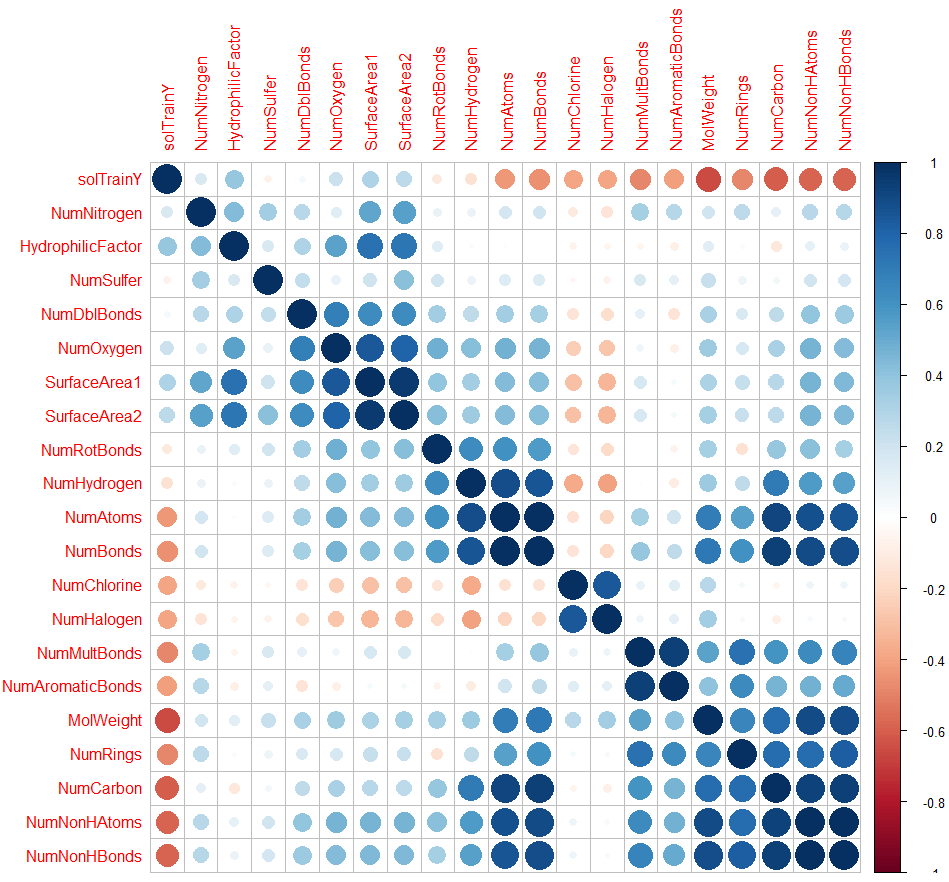
\includegraphics[scale=0.7]{fig/corrplot}
		\caption{Matriz de Correlação entre os \textit{predictors} e a saída representada com círculos.}
		\label{fig:Figura 1}
	\end{figure}
	\newpage
	\begin{figure}[!h]
		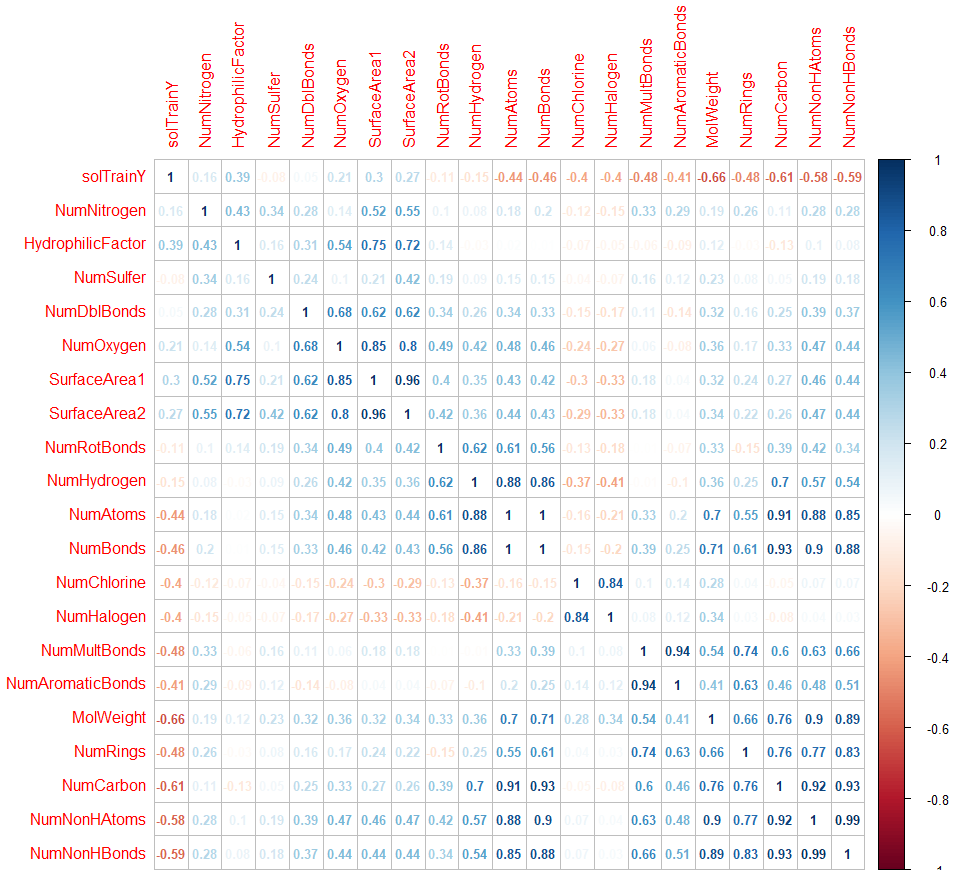
\includegraphics[scale=0.7]{fig/corrplotNumber}
		\caption{Matriz de Correlação entre os \textit{predictors} e a saída representado em valores.}
		\label{fig:Figura 2}
	\end{figure}
	Podemos verificar que existem muitos pares de \textit{predictors} fortemente correlacionados, que deverão e serão retirados posteriormente para a regressão linear. Além disso, incluímos a saída para verificar se possui algum \textit{predictor} correlacionado a saída e podemos verificar que existem alguns preditores inversamente proporcionais a saída, como o peso molecular. Essa observação é coerente, tendo em vista que quanto maior a molécula, mais difícil ela é de se dissolver.
	\newpage
	\begin{center}
		\section*{Parte 1}
	\end{center}
	Para fazermos um modelo de regressão linear ordinário, devemos primeiramente levar em conta o nosso \textit{dataset}. Devemos analisar se as correlações entre os \textit{predictors} e retirar os que são muito correlacionados. Dado que utilizamos a formula $(X^{T} X)^{-1}X^{T}y$, onde $X$ é a matriz dos \textit{predictors} e $y$ é o vetor resposta, o termo $(X^{T} X)^{-1}$, que é proporcional a matriz de covariância dos \textit{predictors}, só vai possuir inversa única quando os termos não forem colineares e numero de amostras for maior que os de \textit{predictors}. Sendo assim, nosso primeiro passo será retirar os \textit{predictors} que tem correlação maior que 0.9.
	\begin{minted}[tabsize=0,breaklines]{R}
	corThresh <- .9;
	tooHigh <- findCorrelation(cor(solTrainXtrans), corThresh);
	corrPred <- names(solTrainXtrans)[tooHigh];
	length(tooHigh)
	corrPred
	
	trainXfiltered <- solTrainXtrans[, -tooHigh];
	testXfiltered <- solTestXtrans[, -tooHigh];
	\end{minted}
	Após executado o código, identificamos 38 \textit{predictors} com correlação maior que 0.9. Esses \textit{predictors} foram então descartados para podermos aplicarmos a regressão linear. O próximo passo é aplicar a função \textit{\textbf{lm}}. Para aplicar essa função, é preciso que o \textit{output} esteja no mesmo \textit{dataset} que os \textit{predictors} que vão ser analisados. Depois disso, aplicamos a função e depois verificamos a eficiência dela com o \textit{test set} utilizando a função \textit{\textbf{predict}}:
	\begin{minted}[tabsize=0,breaklines]{R}
	set.seed(200)
	trainingData <- trainXfiltered
	trainingData$solubility <- solTrainY
	
	lmFiltered <-lm(Solubility ~ ., data = trainingData)
	lmPred1 <- predict(lmFiltered, testXfiltered)
	
	lmValues1 <- data.frame(obs = solTestY, pred = lmPred1)
	defaultSummary(lmValues1)
	\end{minted}
	\begin{center}
		\begin{tabular}{c c}
			\multicolumn{2}{ c }{Resultados da regressão linear ordinária aplicada ao \textit{test set}}\\
			\hline
			RMSE & $R^{2}$ \\
			\hline
			0.7601790 & 0.8669049
		\end{tabular}
	\end{center}
	Desse modo, conseguimos obter um modelo de regressão linear ordinário para o nosso \textit{dataset}. O RMSE e o $R^{2}$ para esse modelo é 0.760 e 86,7\%, respectivamente. Agora, verificaremos as medidas utilizando um \textit{10-fold cross validation}. Para isso, utilizaremos outra função, a \textit{\textbf{train}}:
	\begin{minted}[tabsize=0,breaklines]{R}
	fold10 <- trainControl(method = "cv", number = 10);
	
	lmTrain10 <- train(trainXfiltered, solTrainY, method = "lm", trControl = fold10);
	lmTrain10
	
	plotlm10ob<-xyplot(solTestY ~ predict(lmTrain10,testXfiltered), type = c("p", "g"), xlab = "Predicted", ylab = "Observed", col = "blue")
	plotlm10re<-xyplot(resid(lmTrain10) ~ predict(lmTrain10,testXfiltered), type = c("p", "g"), xlab = "Predicted", ylab = "Residuals", col = "blue")

	print(plotlm10ob, pos = c(0.0,0.0,0.5,1), more = TRUE)
	print(plotlm10re, pos = c(0.5,0.0,1,1), more = FALSE)
	\end{minted}
	\begin{center}
		\begin{tabular}{c c}
			\multicolumn{2}{ c }{Resultados da regressão linear ordinária utilizando \textit{10-fold cross validation}}\\
			\hline
			RMSE & $R^{2}$ \\
			\hline
			0.691249 & 0.8863239
		\end{tabular}
	\end{center}
	\begin{figure}[h!]
		\begin{center}
			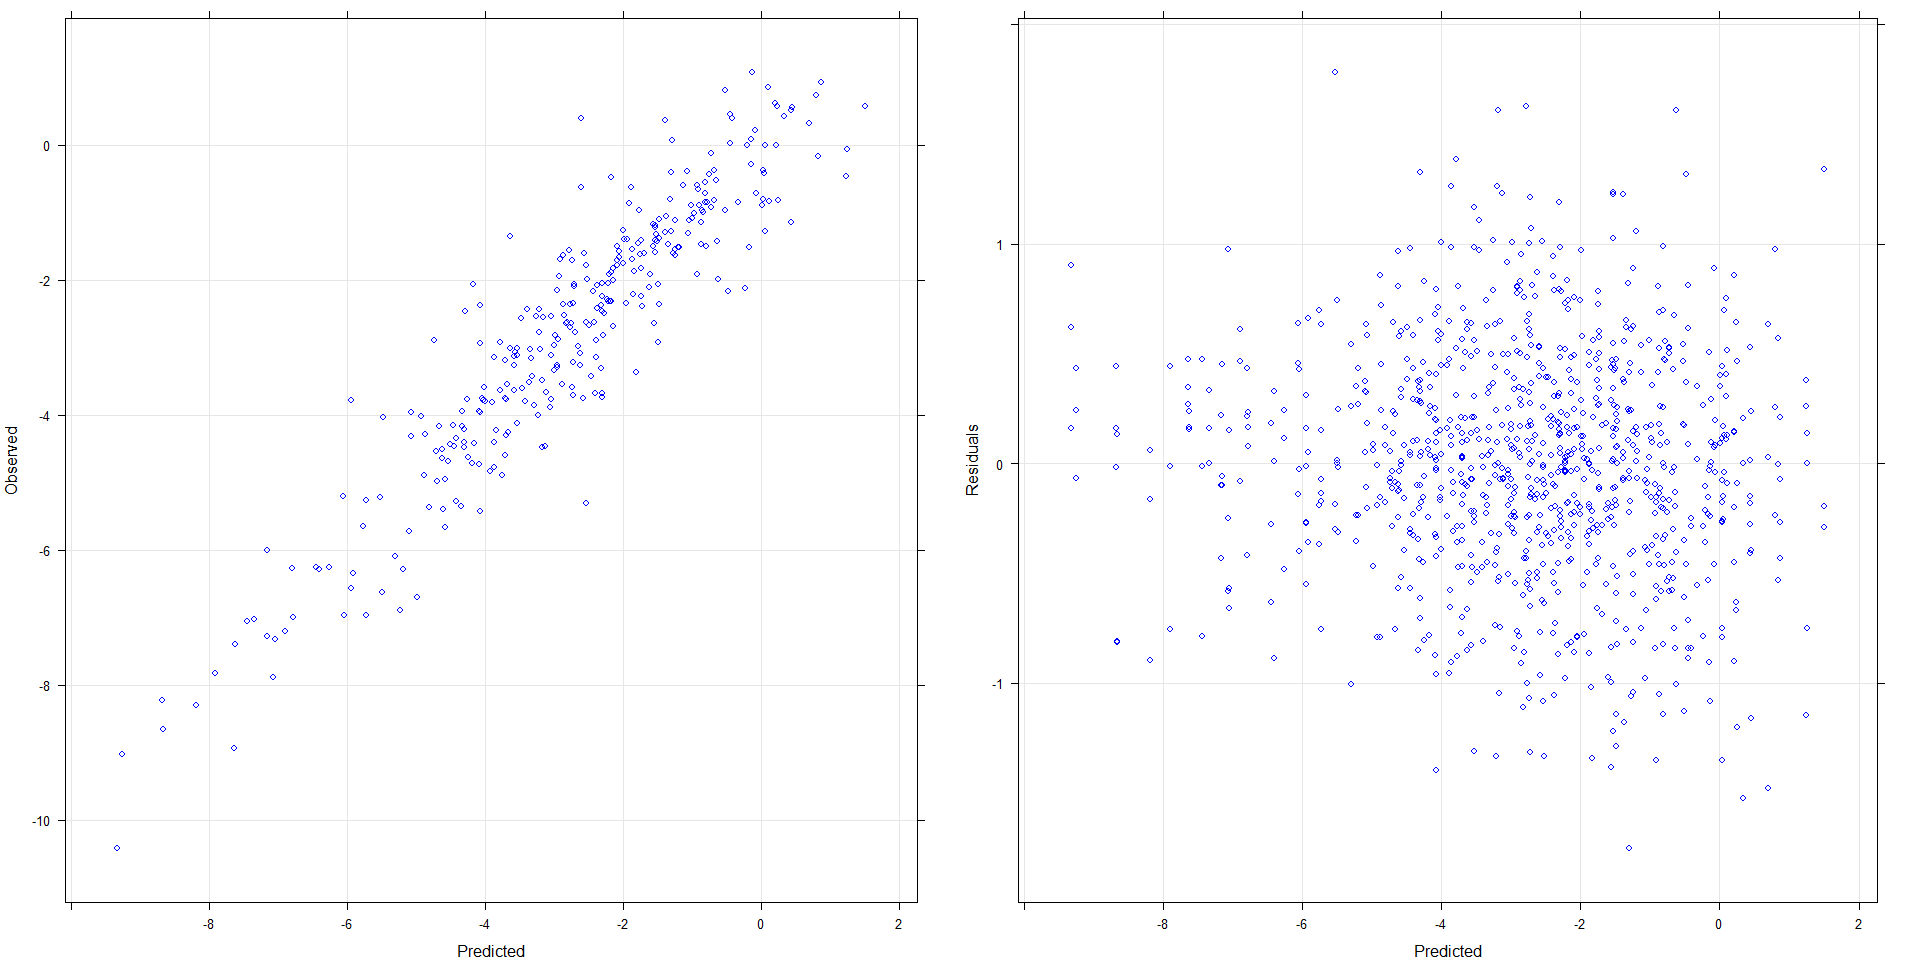
\includegraphics[scale=0.3]{fig/lmplot}
			\caption{Esquerda: Grafico dos valores observados pelo os previstos pelo modelo de regressão linear. Direita: Gráfico dos resíduos do modelo de regressão linear pelo valor previsto.}
		\end{center}
	\label{fig:Figura 3}
	\end{figure}
	Verificamos então o RMSE e o $R^{2}$ medido pelo \textit{10-fold cross validation}. Obtemos 0.69 e 88,6\%, respectivamente. Comparados com os valores dados pela verificação pelo \textit{test set}, 0.760 e 86,7\%, podemos concluir que ambas verificações tem eficiência bem parecida para esse \textit{dataset}. No nosso caso, temos muitas amostras, de modo que usar um \textit{test set} não é problema, mas no caso de \textit{datasets} menores, utilizar \textit{K-fold cross validation} pode ser a única opção.\\
	Analisando a \autoref{fig:Figura 3}3, podemos concluir que o modelo está coerente, pois verificamos a linearidade entre o previsto e o observado do lado esquerdo, e do lado direito vemos que os pontos de resíduo estão dispersos em torno do 0, de modo que seu somatório deve dar próximo disso.
	\begin{center}
		\section*{Parte 2}
	\end{center}
	Nessa parte, devemos fazer um modelo de regressão linear penalizado $L_{2}$.
	A regressão linear penalizada foi introduzida com o intuito de consertar algumas dificuldades geradas pela regressão linear ordinária. Essas dificuldades são, principalmente, o \textit{overfitting}, que é uma visão otimista dos dados, gerando um modelo "viciado", e os preditores correlatos, que são tirados para que o modelo funcione. Esses casos são gerados pois as vezes o parâmetro da regressão linear ordinária pode estar \textit{inflated}. O modelo de regressão linear penalizada de \textit{\textbf{Ridge}} resolve isso aplicando um termo de penalização ao quadrado na função \textit{hat}.
	Para aplicarmos a regressão linear penalizada, usaremos o modelo de \textit{\textbf{Ridge}}. Primeiramente, iremos aplicar a função \textit{\textbf{train}} com \textit{10-fold cross validation} para acharmos o melhor valor de lambda. Além disso, pre-processamos os dados para eles ficaram normalizados e centralizados. Dessa forma, os contornos da função do erro fica mais redondo e espaçado, facilitando na hora de aplicarmos \textit{Ridge}. Se não normalizassemos os valores, teriamos fronteiras mais próximas e elípticas.
	\begin{minted}[tabsize=0,breaklines]{R}
	ridgeGrid <- data.frame(.lambda = seq(0, .1, length = 15))
	set.seed(200)
	ridgeRegFit <- train(solTrainXtrans, solTrainY, method = "ridge", tuneGrid = ridgeGrid, trControl = fold10,preProc = c("center", "scale"))
	ridgeRegFit
	plot(ridgeRegFit, xlab = "Penalty", ylab = "RMSE (Cross Validation)")
	\end{minted}
	\begin{center}	
		\begin{tabular}{c c c}
			\multicolumn{3}{ c }{Resultados da regressão linear Ridge $L_{2}$}\\
			\hline
			lambda      & RMSE      & $R^{2}$\\
			\hline         
			0.000000000 & 0.6940069 & 0.8838059 \\ 
			0.007142857 & 0.6824777 & 0.8879880 \\
			0.014285714 & 0.6769873 & 0.8902612 \\
			\textbf{0.021428571} & \textbf{0.6755135} & \textbf{0.8911183} \\
			0.028571429 & 0.6758089 & 0.8913708 \\
			0.035714286 & 0.6770933 & 0.8913038 \\
			0.042857143 & 0.6790107 & 0.8910488 \\
			0.050000000 & 0.6813715 & 0.8906763 \\
			0.057142857 & 0.6840645 & 0.8902281 \\
			0.064285714 & 0.6870200 & 0.8897302 \\
			0.071428571 & 0.6901922 & 0.8891999 \\ 
			0.078571429 & 0.6935498 & 0.8886490 \\
			0.085714286 & 0.6970709 & 0.8880856 \\ 
			0.092857143 & 0.7007396 & 0.8875153  \\
			0.100000000 & 0.7045442 & 0.8869424 \\
		\end{tabular}
		\begin{figure}[h!]
			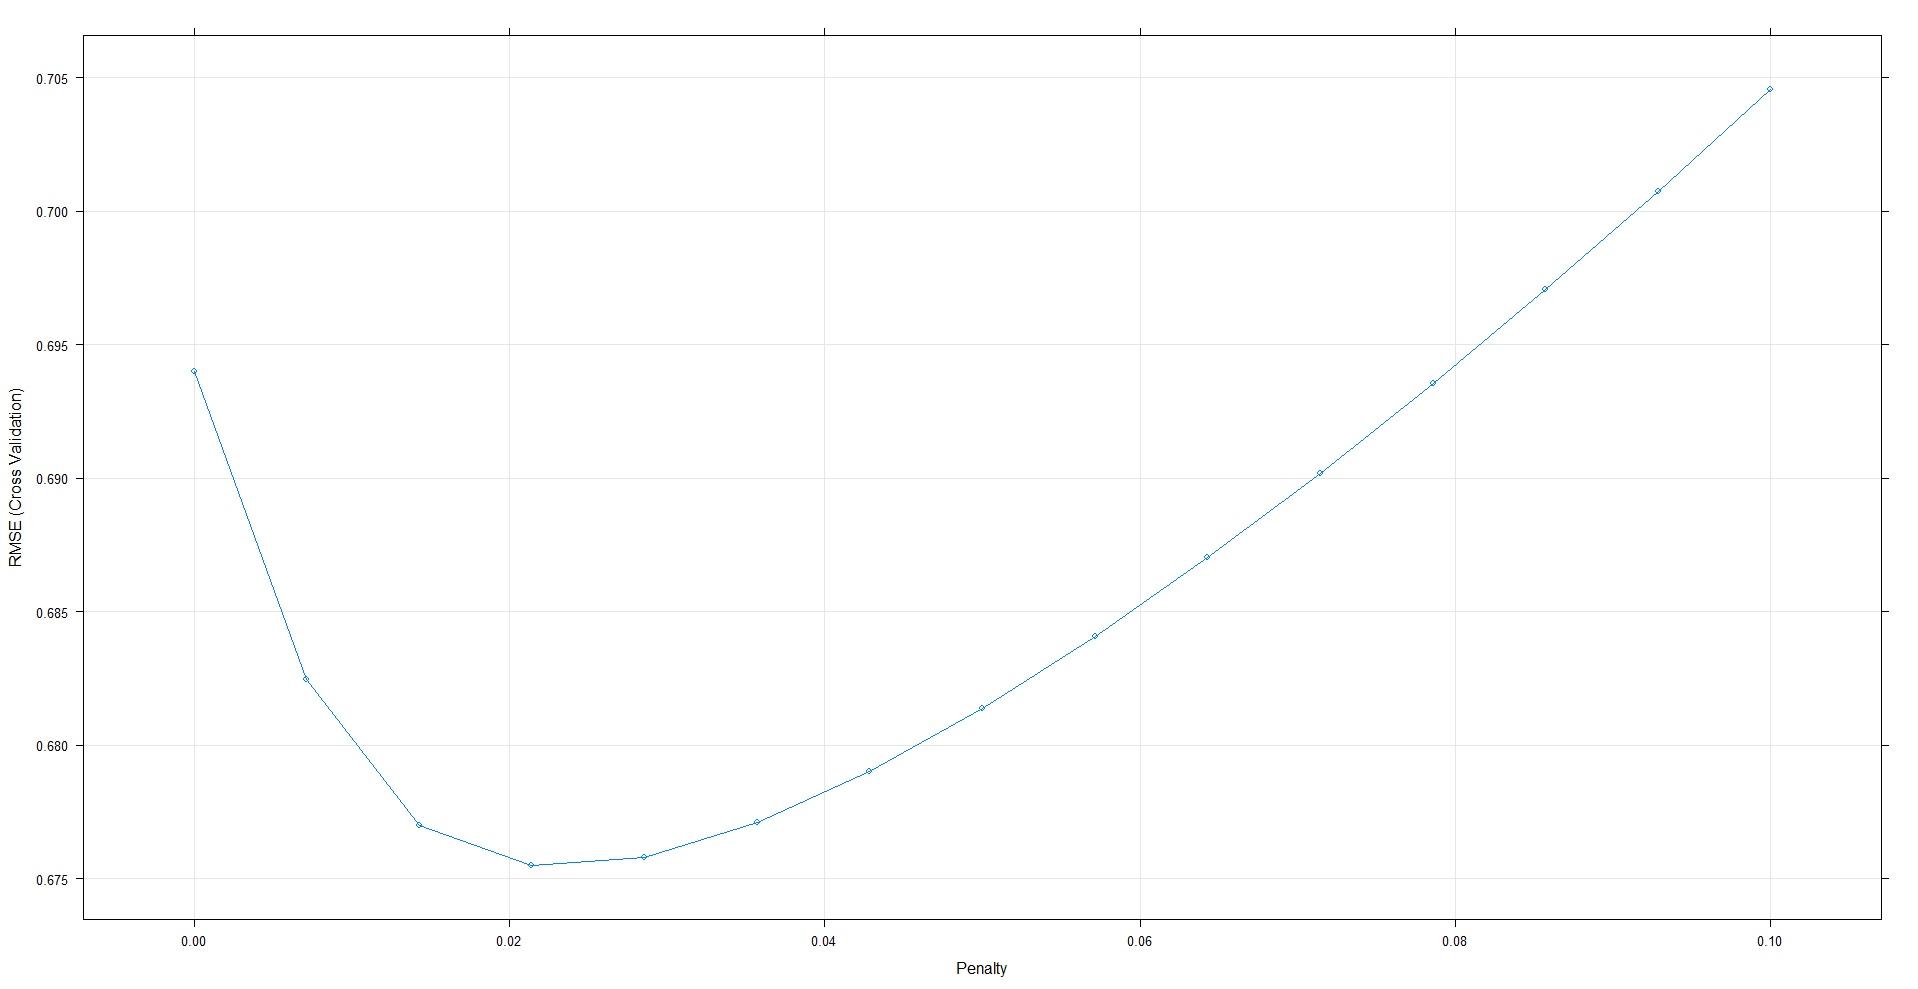
\includegraphics[scale=0.4]{fig/ridgeRMSElambda}
			\caption{Gráfico da RMSE x Valores de lambda na regressão linear Ridge}
			\label{fig:Figura 4}
		\end{figure}
	\end{center}
	Conseguimos identificar que o menor valor de RMSE dado esses 15 lambda é 0.6755135, que corresponde ao $\lambda$ = 0.021428571. Podemos observar na \autoref{fig:Figura 4}, a tendência que a curva RMSE x $\lambda$ tem de decrescer primeiro e depois aumentar. Para melhorar a eficiência, podíamos acrescentar mais lambdas perto do valor ótimo achado, de modo que teríamos um melhor ajuste fino. Agora, com o modelo já feito, iremos testar no \textit{test set} e compararemos os valores de RMSE e $R^{2}$
	\begin{minted}[tabsize=0,breaklines]{R}
	lmRidgePred <- predict(ridgeRegFit, solTestXtrans)
	ridge.df <- data.frame(pred = lmRidgePred, obs = solTestY)
	defaultSummary(ridge.df)
	\end{minted}
	\begin{center}
		\begin{tabular}{c c c}
			\multicolumn{2}{ c }{Resultados da regressão linear Ridge $L_{2}$ aplicada ao \textit{test set}}\\
			\hline
			lambda & RMSE & $R^{2}$ \\
			\hline
			0.021428571 & 0.7218669 &  0.8800143
		\end{tabular}
	\end{center}
	Comparando os resultados do RMSE e $R^{2}$ do \textit{test set} com os feitos por \textit{cross validation}, podemos concluir que o modelo com \textit{cross validation} estava sendo otimista, já que tem uma diferença considerável do RMSE dele (0.6755135) para o feito com o \textit{test set} (0.7218669). Esse resultado é coerente, pois a verificação por \textit{cross validation} usa apenas o conjunto de treino, de modo que ela é um pouco menos eficaz que uma verificação via \textit{test set}.
	\begin{center}
		\section*{Parte 3}
	\end{center}
	Nesse passo, iremos aplicar um modelo de regressão linear PCR ou PLS. A PCR (\textit{Principal Componente Regression}) é uma regressão que resolve os problemas de correlação entre os preditores utilizando PCA(\textit{Principal Component Analysis}). Pela natureza do PCA, de garantir que nenhum preditor tem relação entre si, ele é um ótimo modelo. Contudo, ele não leva em consideração nenhum aspecto da saída, de modo que se os preditores não tiverem uma variância relacionada a saída, ele não vai ser eficiente. Tendo em vista esse problema, e como nós foi sugerido no livro, utilizaremos o PLS.
	O PLS (\textit{Partial Least Squares}) surgiu com o \textit{nonlinear iterative partial least squares algorithm} (NIPALS), que linearizava modelos que eram não-lineares em seus parâmetros. Ele funciona de modo que consegue levar em consideração as variâncias dos preditores enquanto requisita que essas componentes tenham máxima correlação com as saídas, enquanto reduz sua dimensão para fazer a regressão. Desse modo, esse procedimento é chamado de \textit{\textbf{supervisionado}}(\textit{supervised dimension reduction procedure}).
	Utilizando a função \textit{\textbf{Train}}, iremos desenvolver a PLS:
	\begin{minted}[tabsize=0,breaklines]{R}
	set.seed(200)
	plsTune <- train(solTrainXtrans, solTrainY, method = "pls", tuneLength = 25, trControl = fold10, preProc = c("center", "scale"))
	plsTune
	plot(plsTune, xlab = "Number of components", ylab = "RMSE (Cross Validation)")
	\end{minted}
	\begin{center}
		\begin{tabular}{c c c}
			\multicolumn{2}{ c }{Resultados da PLS com \textit{10-fold Cross Validation}}\\
			\hline
			 Nº of components & RMSE  & $R^{2}$   \\
			 \hline    
			1   &  1.2849536  & 0.6090610    \\
			2   &  1.0549228  & 0.7335585    \\
			3   &  0.9369236  & 0.7901420    \\
			4   &  0.8623083  & 0.8217281    \\
			5   & 0.8191507   & 0.8387654    \\
			6   &  0.7844736  & 0.8528814    \\
			7   &  0.7573361  & 0.8630147    \\
			8   &  0.7415002  & 0.8685131    \\
			9   &  0.7327694  & 0.8725782    \\
			10  &   0.7195060 & 0.8774698   \\
			11  &   0.7127775 & 0.8790996   \\
			12  &   0.7076509 & 0.8809095   \\
			13  &   0.7032763 & 0.8822672   \\
			14  &   0.7013346 & 0.8830113   \\
			15  &   0.6966530 & 0.8844692   \\
			16  &   0.6950322 & 0.8850275   \\
			17  &   0.6929195 & 0.8854159   \\
			\textbf{18}  &   \textbf{0.6896578} & \textbf{0.8866734}   \\
			19  &   0.6901727 & 0.8863902   \\
			20  &   0.6909659 & 0.8860459   \\
			21  &   0.6943647 & 0.8849180   \\
			22  &   0.6965550 & 0.8838458   \\
			24  &   0.6971807 & 0.8834652   \\
			25  &   0.6999703 & 0.8825882   \\
		\end{tabular}
		\newpage
		\begin{figure}[h!]
			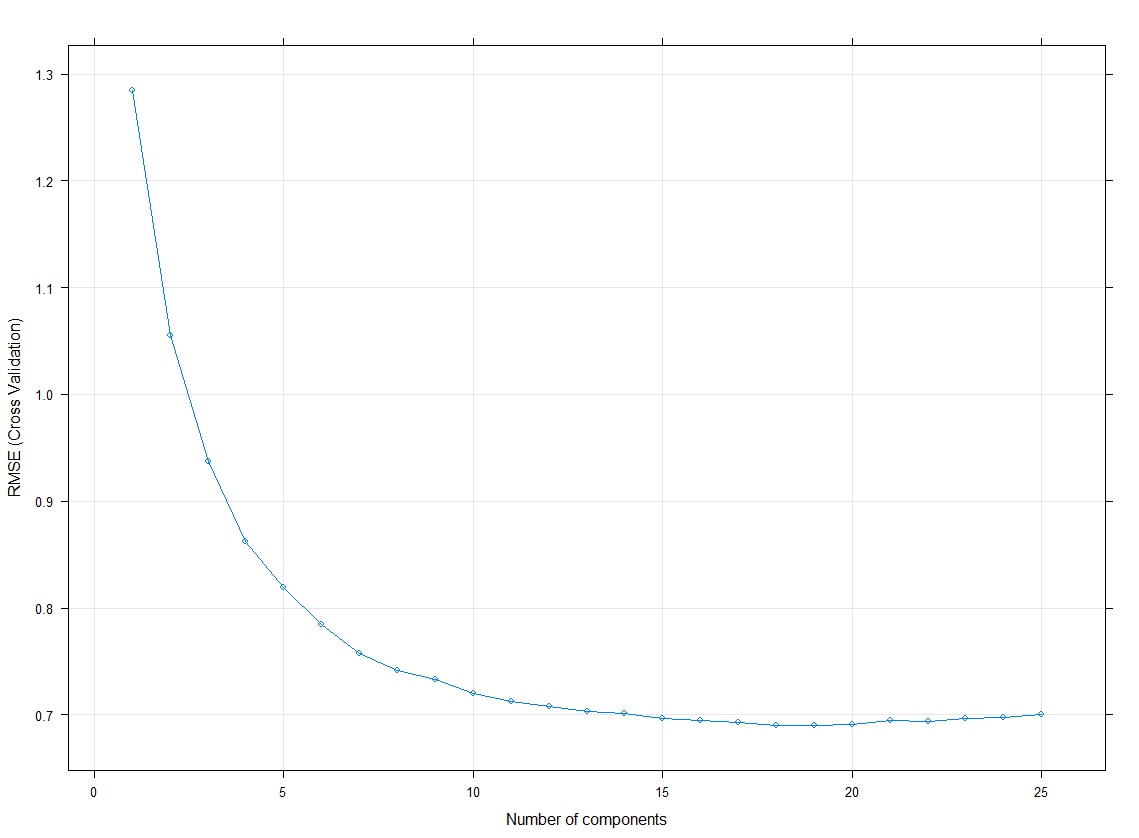
\includegraphics[scale=0.6]{fig/plsRMSEncomp}
			\caption{Gráfico da RMSE x Numeros de componentes na PLS}
			\label{fig:Figura 5}
		\end{figure}
	\end{center}
	Na \autoref{fig:Figura 5} temos o gráfico dos erros pelo número de componentes. Percebemos que ela atinge o minimo aproximadamente com 18 componentes, o que condiz com o resultado achado na função \textit{\textit{train}}. Agora, iremos aplicar essa regressão no \textit{test set} e medir sua eficiência.
	\begin{minted}[tabsize=0,breaklines]{R}
	plsPred <- predict(plsTune, solTestXtrans)
	pls.df <- data.frame(pred = plsPred, obs = solTestY)
	defaultSummary(pls.df)
	\end{minted}
	\begin{center}
		\begin{tabular}{c c c}
			\multicolumn{2}{ c }{Resultados da PLS aplicada ao \textit{test set}}\\
			\hline
			Nº Components & RMSE & $R^{2}$ \\
			\hline
			18 & 0.7296398 & 0.8772282
		\end{tabular}
	\end{center}
	Com isso, temos um valor razoavelmente maior de RMSE comparado ao \textit{cross validation}, como temos tido durante todo esse trabalho (que é o usual).
	\begin{center}
		\section*{Análise final}
	\end{center}
	Para fechar, iremos fazer uma analise comparativa dos 3 modelos de regressão linear abaixo, e tentar verificar se os resultados estão coerentes.
	\vskip0.4cm
	\begin{center}
		\begin{tabular}{c c c c}
			\multicolumn{4}{ c }{Resultados das regressões lineares aplicadas no trabalho}\\
			\hline
			  & RLO & Ridge & PLS \\
			\hline
			RMSE    & 0.7601790 & 0.7218669 & 0.7296398 \\
			$R^{2}$ & 0.8669049 & 0.8800143 & 0.8772282 
		\end{tabular}
	\end{center}
	Percebemos que os valores de $R^{2}$ são semelhantes e relativamente altos, mas nem tanto. Desse modo, podemos concluir que os modelos correspondem bem e não possuem \textit{overfitting}, que é o principal indicativo de altas porcentagens de $R^{2}$. Quanto ao RMSE, o fato mais curioso seria a melhor eficiência da regressão \textit{Ridge} em relação a PLS, mesmo que por pouco. Como a PLS é um modelo mais robusto e supervisionado, a tendência seria de achar que sua eficiência seria melhor que a \textit{Ridge}. Contudo, como constatado no livro-texto da disciplina, o PLS perde rendimento a medida que a quantidade de preditores aumenta. Desse modo, como possuimos muitos preditores, a PLS acaba perdendo sua eficiência a ponto da Regressão \textit{Ridge} ser melhor que ela.
\end{document}